\documentclass[tikz,11pt]{standalone}
\usepackage{newtxtext,newtxmath}

\usetikzlibrary{shapes.misc,shapes.arrows,shapes.multipart}
\usetikzlibrary{positioning}
\usetikzlibrary{calc}

\tikzset{
    between/.style args={#1 and #2}{at = ($(#1)!0.5!(#2)$)},
    universe/.style = {draw, rounded rectangle, 
                       minimum width=10cm, minimum height=7cm,
    },
    system/.style = {draw, rounded rectangle, anchor=west, 
                     minimum width=2cm, minimum height=2cm
    },
    environment/.style = {draw, rounded rectangle, anchor=east,
                          minimum width=6cm, minimum height=5cm
    },
    interaction arrow/.style = {double arrow, minimum height=1.5cm, 
                                double arrow head extend=1ex, fill=black!10,
    },
}

\begin{document}
    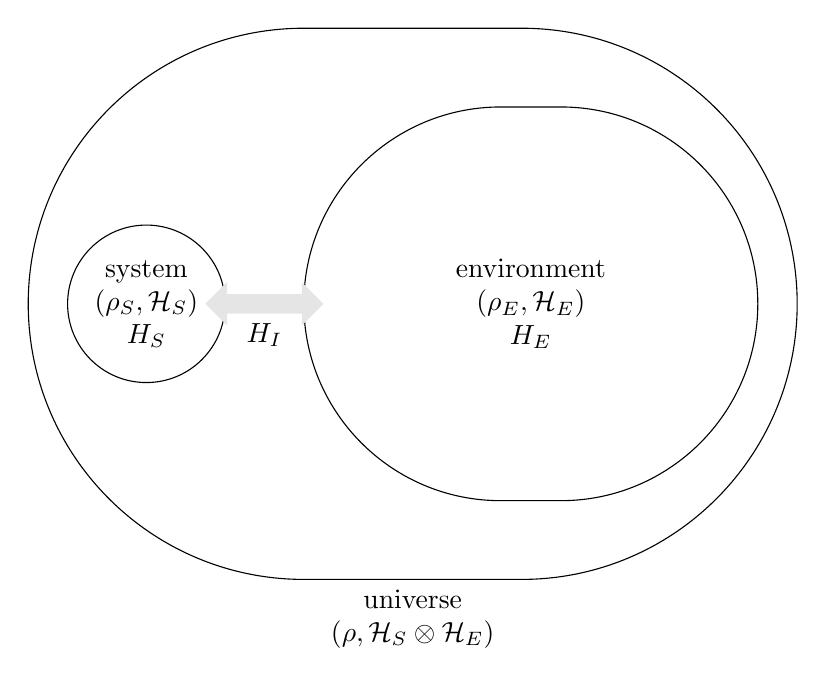
\begin{tikzpicture}[every text node part/.style={align=center}]
        \node (u) [universe, 
                   label={below:{
                   universe\\ $(\rho, \mathcal{H}_S \otimes \mathcal{H}_E)$}
                   }] {};
        \node (s) [system, right=0.5cm of u.west] 
                  {system \\ $(\rho_S, \mathcal{H}_S)$ \\ $H_S$};
        \node (e) [environment, left=0.5cm of u.east] 
                  {environment \\ $(\rho_E, \mathcal{H}_E)$ \\ $H_E$};
        \node (i) [interaction arrow, between=s.east and e.west, 
                   label={below:$H_I$}] {};
    \end{tikzpicture}
\end{document}
